% \documentclass[aspectratio=169,notes]{beamer}
\documentclass[aspectratio=169]{beamer}
\usetheme[faculty=phil]{fibeamer}
\usepackage{polyglossia}
\setmainlanguage{english} %% main locale instead of `english`, you
%% can typeset the presentation in either Czech or Slovak,
%% respectively.
\setotherlanguages{russian} %% The additional keys allow
%%
%%   \begin{otherlanguage}{czech}   ... \end{otherlanguage}
%%   \begin{otherlanguage}{slovak}  ... \end{otherlanguage}
%%
%% These macros specify information about the presentation
\title[Introduction to Robotics (In2Ro)]{Introduction to Robotics, Homework Hard 1} %% that will be typeset on the
\subtitle{Manipulation: UR5, IIMT CI-05, Limo CoRoT arm 
\\ A pallet of cubes from a taught frame \\ \ } %% title page.
\author{Oleg Bulichev}
%% These additional packages are used within the document:
\usepackage{ragged2e}  % `\justifying` text
\usepackage{booktabs}  % Tables
\usepackage{tabularx}
\usepackage{tikz}      % Diagrams
\usetikzlibrary{calc, shapes, backgrounds, trees, positioning, arrows.meta}
\usetikzlibrary{decorations.pathreplacing,calligraphy,calc,graphs}
\usepackage{amsmath, amssymb}
\usepackage{url}       % `\url`s
\usepackage{listings}  % Code listings
\usepackage{floatrow}
\usepackage{subcaption}
\usepackage{mathtools}
\usepackage{todonotes}
\usepackage{fontspec}
\usepackage{multicol}
\usepackage{pdfpages}
\usepackage{wrapfig}
\usepackage{qrcode}
\usepackage{animate}
\usepackage{booktabs}
\usepackage{multirow}
\usepackage{graphicx}
\usepackage{colortbl}

\graphicspath{{resources/}}
\frenchspacing

\setbeamertemplate{caption}{\raggedright\insertcaption\par}
\usetikzlibrary{graphs}

% \usepackage[backend=biber,style=ieee,autocite=footnote]{biblatex}
% \addbibresource{biblio.bib}
% \DefineBibliographyStrings{english}{%
%   bibliography = {References},}

\newcommand{\oleg}[2][] {\todo[color=red, #1] {OLEG:\\ #2}}
\newcommand{\fbckg}[1]{\usebackgroundtemplate{\includegraphics[width=\paperwidth]{#1}}}%frame background

\usepackage[framemethod=TikZ]{mdframed}
\newcommand{\dbox}[1]{
\begin{mdframed}[roundcorner=3pt, backgroundcolor=yellow, linewidth=0]
\vspace{1mm}
{#1}
\vspace{1mm}
\end{mdframed}
}

\begin{document}
\setlength{\abovedisplayskip}{0pt}
\setlength{\belowdisplayskip}{0pt}
\setlength{\abovedisplayshortskip}{0pt}
\setlength{\belowdisplayshortskip}{0pt}

\fbckg{fibeamer/figs/title_page.png}
\frame[c]{\setcounter{framenumber}{0}
    \usebeamerfont{title}%
    \usebeamercolor[fg]{title}%
    \begin{minipage}[b][6.5\baselineskip][b]{\textwidth}%
        \textcolor{black}{\raggedright\inserttitle}
    \end{minipage}
    % \vskip-1.5\baselineskip

    \usebeamerfont{subtitle}%
    \usebeamercolor[fg]{framesubtitle}%
    \begin{minipage}[b][3\baselineskip][b]{\textwidth}
        \raggedright%
        \insertsubtitle%
    \end{minipage}
    \vskip.25\baselineskip
}

\fbckg{fibeamer/figs/common.png}

\begin{frame}[t]{What this homework is}
\framesubtitle{Make an arm place cubes on a grid it has never been shown}
    The arm builds a $3\times3$ pallet of cubes on a table. You do not read the nine cell
    positions off the controller one by one: you compute them in a coordinate frame that you
    teach the robot by touching three points, and you check every pose in a simulator of
    your own before the real arm moves.
    \medskip

    \begin{itemize}
        \item Choose \textbf{one} arm: UR5, IIMT CI-05, or the Limo CoRoT arm.
        \item Name the arm on the first page of your report.
        \item If you choose the Limo arm, use the Limo robot in Homework Hard 2 as well.
    \end{itemize}
\end{frame}

\begin{frame}[t]{Four tasks, one chain}
\framesubtitle{Each task produces the input of the next one}
    \centering
    \vspace{2mm}
    \begin{tikzpicture}[
        box/.style={draw, rounded corners=3pt, minimum width=3.0cm, minimum height=1.4cm,
                    align=center, fill=blue!8},
        arr/.style={-{Stealth[length=2.5mm]}, thick}]
        \node[box] (a) {Task 1\\ Simulator\\ from DH};
        \node[box, right=5mm of a] (b) {Task 2\\ Work frame\\ from 3 points};
        \node[box, right=5mm of b] (c) {Task 3\\ Grid, IK,\\ reachability};
        \node[box, right=5mm of c] (d) {Task 4\\ Program\\ on the robot};
        \draw[arr] (a) -- (b);
        \draw[arr] (b) -- (c);
        \draw[arr] (c) -- (d);
    \end{tikzpicture}
    \medskip

    \begin{minipage}{0.92\textwidth}
        \raggedright
        The simulator (Task 1) checks the grid (Task 3). The grid is written in the work
        frame (Task 2). The program (Task 4) runs the same grid on the real arm, and you
        measure how well the real arm repeats it.
    \end{minipage}
\end{frame}

\begin{frame}[t]{UR5 (Universal Robots)}
    \begin{minipage}[t]{0.55\textwidth}
        \vspace{0pt}
        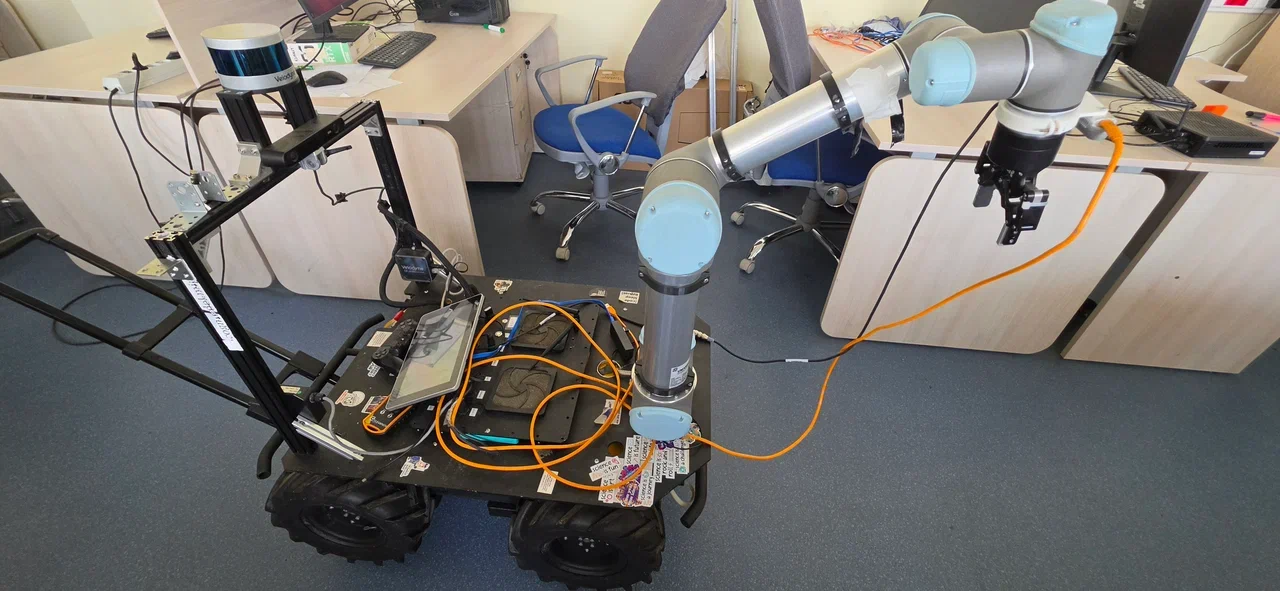
\includegraphics[width=\linewidth]{robot_ur5.png}
    \end{minipage}
    \hfill
    \begin{minipage}[t]{0.43\textwidth}
        \vspace{0pt}
        \small
        \textbf{What it is.} Six-joint collaborative arm, payload 5\,kg, reach 850\,mm; ours
        has a two-finger gripper.
        \smallskip

        \textbf{Programming.} On the teach pendant: Move blocks with waypoints, a Loop and
        Features (coordinate frames). The pendant shows the TCP pose.
        \smallskip

        \textbf{Documentation.} \url{universal-robots.com/manuals}; the UR page ``DH parameters
        for calculations of kinematics and dynamics''.
    \end{minipage}
\end{frame}

\begin{frame}[t]{IIMT CI-05}
    \begin{minipage}[t]{0.27\textwidth}
        \vspace{0pt}
        \centering
        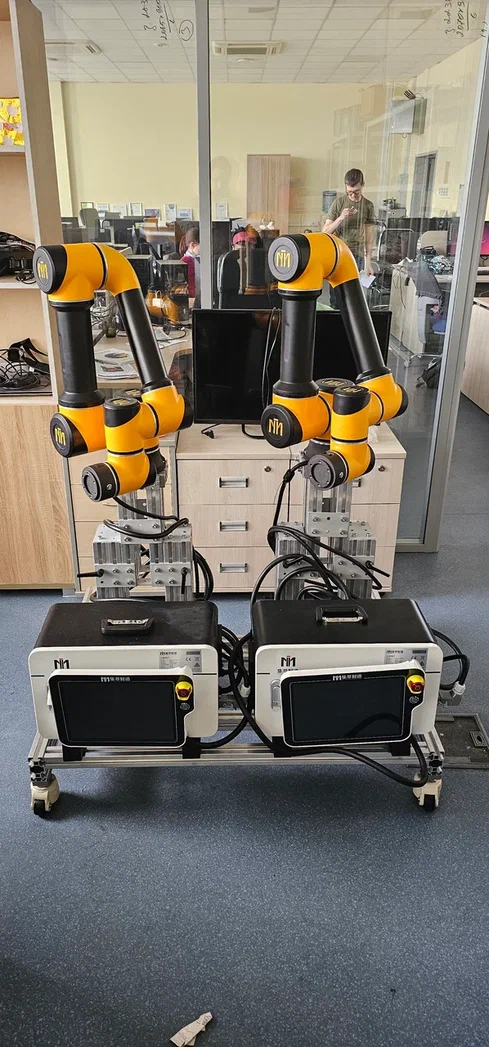
\includegraphics[height=5.6cm,width=\linewidth,keepaspectratio]{robot_iimt.png}
    \end{minipage}
    \hfill
    \begin{minipage}[t]{0.70\textwidth}
        \vspace{0pt}
        \small
        \textbf{What it is.} Six-joint collaborative arm built like the UR5 but with its own
        dimensions: payload 5\,kg, working radius 900\,mm, mass 20.4\,kg, repeatability
        $\pm0.03$\,mm, joints $\pm360^\circ$. Two units, each with its own controller and
        pendant.
        \smallskip

        \textbf{Programming.} On its teach pendant, with waypoints, a loop and a user
        coordinate frame, as on the UR5.
        \smallskip

        \textbf{Documentation.} \url{iimtcobot.com/iimt-ci-05-robotic-arm.html}; on the
        downloads page of the same site: the CI-05 outline drawing.
    \end{minipage}
\end{frame}

\begin{frame}[t]{Limo CoRoT arm (myCobot 280)}
    \begin{minipage}[t]{0.27\textwidth}
        \vspace{0pt}
        \centering
        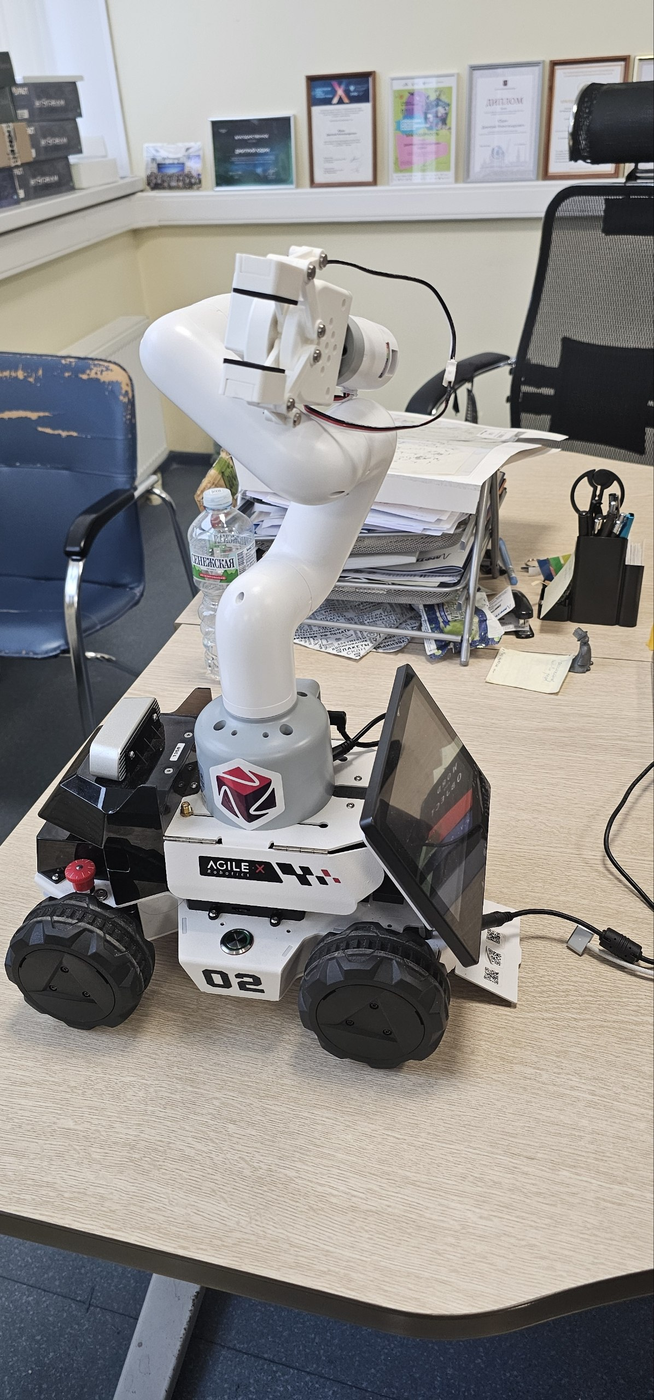
\includegraphics[height=5.6cm,width=\linewidth,keepaspectratio]{robot_limo.png}
    \end{minipage}
    \hfill
    \begin{minipage}[t]{0.70\textwidth}
        \vspace{0pt}
        \small
        \textbf{What it is.} A small six-joint arm on the Limo base: reach 280\,mm, payload
        250\,g, repeatability $\pm0.5$\,mm, adaptive gripper; use light cubes. Joint limits
        J1 $\pm168^\circ$, J2 $\pm135^\circ$, J3 $\pm150^\circ$, J4 $\pm145^\circ$, J5
        $\pm165^\circ$, J6 $\pm180^\circ$.
        \smallskip

        \textbf{Programming.} No pendant: a Python script on the Limo computer sends joint
        angles (degrees) or poses (millimetres, degrees) through \texttt{pymycobot}; see
        \texttt{limo\_arm.py}.
        \smallskip

        \textbf{Documentation.} \url{github.com/elephantrobotics/LIMO-Cobot-docs}, folder
        \texttt{mycobot\_280\_M5(2023)en}: parameters, Python API, DH figure.
    \end{minipage}
\end{frame}

\begin{frame}[t]{Link dimensions and DH parameters}
\framesubtitle{The numbers for Task 1, in millimetres}
    \footnotesize
    In the standard Denavit--Hartenberg convention joint $i$ has a link length $a_i$ (along the
    common normal of two joint axes), a link twist $\alpha_i$, a joint offset $d_i$ (along the
    joint axis) and a joint angle $\theta_i$, the variable of a revolute joint.
    \smallskip

    \begin{center}
    \begin{tabular}{@{}lrrrrrr@{}}
        \toprule
        & $d_1$ & $a_2$ & $a_3$ & $d_4$ & $d_5$ & $d_6$ \\
        \midrule
        UR5        & 89.159 & $-425$   & $-392.25$ & 109.15 & 94.65 & 82.3 \\
        IIMT CI-05 & 139    & $-394.5$ & $-381$    & 138    & 143   & 103  \\
        Limo arm   & 131.56 & 110.4    & 96        & 64.62  & 73.18 & 48.6 \\
        \bottomrule
    \end{tabular}
    \end{center}
    \smallskip

    UR5 and IIMT: $\alpha = (90^\circ, 0, 0, 90^\circ, -90^\circ, 0)$; every other $a_i$ and $d_i$
    is zero. The Limo arm is given by lengths only; its frames, signs and angle offsets are in
    the vendor figure \texttt{280DH.jpg} of the documentation.
\end{frame}

\begin{frame}[t]{Task 1: Simulator from DH}
\framesubtitle{Build the model of your arm}
    From the previous table, in any language:
    \begin{itemize}
        \item \textbf{FK:} a function from a joint vector $q$ to the $4\times4$ pose of the
              \emph{flange} (the end of the last link) in the base frame. The
              \emph{TCP} (tool centre point: the point of the gripper that touches the cube)
              is the flange pose times a fixed tool transform that you measure.
              Set the same TCP on the controller.
        \item \textbf{Drawing:} the arm as a chain of joint positions for any $q$.
        \item \textbf{Limits:} a warning for a $q$ outside the joint ranges.
    \end{itemize}
    \smallskip

    \texttt{dh\_fk.py}: UR5 reference positions to match to 0.1\,mm; other arms, a tape measure.
\end{frame}

\begin{frame}[t]{Task 1: What to bring}
    \begin{itemize}
        \item The three comparisons with the UR5 reference, or your own proof for another arm.
        \item Drawings of the arm in two poses.
        \item A photo of the real arm in one of those two poses.
    \end{itemize}
\end{frame}

\begin{frame}[t]{Task 2: Work frame from three taught points}
\framesubtitle{The arm must be told where the table is}
    A \emph{work frame} is a coordinate frame glued to the table: an origin and two axes.
    \begin{itemize}
        \item Mark three points: the origin $P_0$, a point $P_1$ on the $+X$ axis, a point
              $P_2$ on the $+Y$ side.
        \item Bring the TCP to each mark and read its position (pendant screen, or
              \texttt{get\_coords()} on the Limo arm).
        \item Compute the $4\times4$ matrix of the work frame in the base frame; show that its
              rotation part is a proper rotation.
        \item UR5 and IIMT: create the three-point frame on the pendant as well and compare.
    \end{itemize}
\end{frame}

\begin{frame}[t]{Task 2: What to bring}
    \begin{itemize}
        \item Photos of the TCP at the three marks.
        \item The three readings and your matrix.
        \item How far its rotation part is from a perfect rotation.
        \item UR5 and IIMT: the difference to the pendant's own frame.
    \end{itemize}
\end{frame}

\begin{frame}[t]{Task 3: Grid and reachability}
\framesubtitle{Nine cells in the work frame}
    The spacing is yours; it must leave room for the gripper fingers.
    \begin{itemize}
        \item Each cell has three poses: \emph{approach} (above), \emph{grasp or place},
              \emph{retreat}. The gripper points down.
        \item Solve the inverse kinematics of every pose in your simulator; say which of the
              solutions you chose and why.
        \item Report for every pose the smallest singular value $\sigma_{\min}$ of the Jacobian
              (closeness to a singularity) and the distance of each joint to its limit.
        \item Replay the whole sequence in the simulator.
    \end{itemize}
\end{frame}

\begin{frame}[t]{Task 3: What to bring}
    \begin{itemize}
        \item A table of the 27 poses, with $\sigma_{\min}$ and the joint margins.
        \item A map of $\sigma_{\min}$ over the grid and a screenshot of the replay.
        \item What you changed when a pose was unreachable or near a singularity.
        \item Limo arm: the reach is only 280\,mm, so choose the grid to fit.
    \end{itemize}
\end{frame}

\begin{frame}[t]{Task 4: Robot program}
\framesubtitle{Ten cycles, then measure}
    Write the pick-and-place program on the controller (Limo arm: a Python script with
    \texttt{limo\_arm.py}) and run ten cycles.
    \begin{itemize}
        \item Straight-line moves for approach and retreat; joint or blended moves between
              cells; a loop for the cycles.
        \item Mark on paper where each cube stands after every cycle; measure the scatter
              with a ruler.
        \item Time one cycle with blend radius $0$ and one with a blend radius above $0$.
              Limo arm: it has no blend radius, so time a cycle that waits at every waypoint
              and a cycle that sends the next command at once.
    \end{itemize}
\end{frame}

\begin{frame}[t]{Task 4: What to bring}
    \begin{itemize}
        \item Screenshots of the program and its waypoints.
        \item Photos of the placed cubes and of the marked paper.
        \item The scatter, the two cycle times, and why they differ.
    \end{itemize}
\end{frame}

\begin{frame}[t]{What you hand in}
\framesubtitle{The same rules for all four tasks}
    \textbf{One report.} The first page names your arm and shows a photo of the setup. For
    each task:
    \begin{itemize}
        \item what you did and why, with the formulas and numbers;
        \item photos of the setup and the result, with a ruler or tape in frame wherever a
              distance is measured;
        \item screenshots of the program or code, printed values and plots;
        \item a table of several runs, and what went wrong and what you changed.
    \end{itemize}
    Code goes as files; the report quotes only what it discusses.
\end{frame}

\fbckg{fibeamer/figs/last_page.png}
\frame[plain]{}

\end{document}
